% \newpage
\section{Evaluation}
\label{sec:evaluation}
In figure \ref{fig:plot1} the raw data of the temperature sensors are plotted with their timestamp. 
The large time deviation of the sensor d39896f013c is particularly striking.
In addition, a stepwise drop in temperature can be seen even before the water bath and it can be seen that the different sensors also show systematic differences in the water temperature.
The slight noise in the measured values also shows that these are point values and not average values.

\begin{figure}
    \centering 
    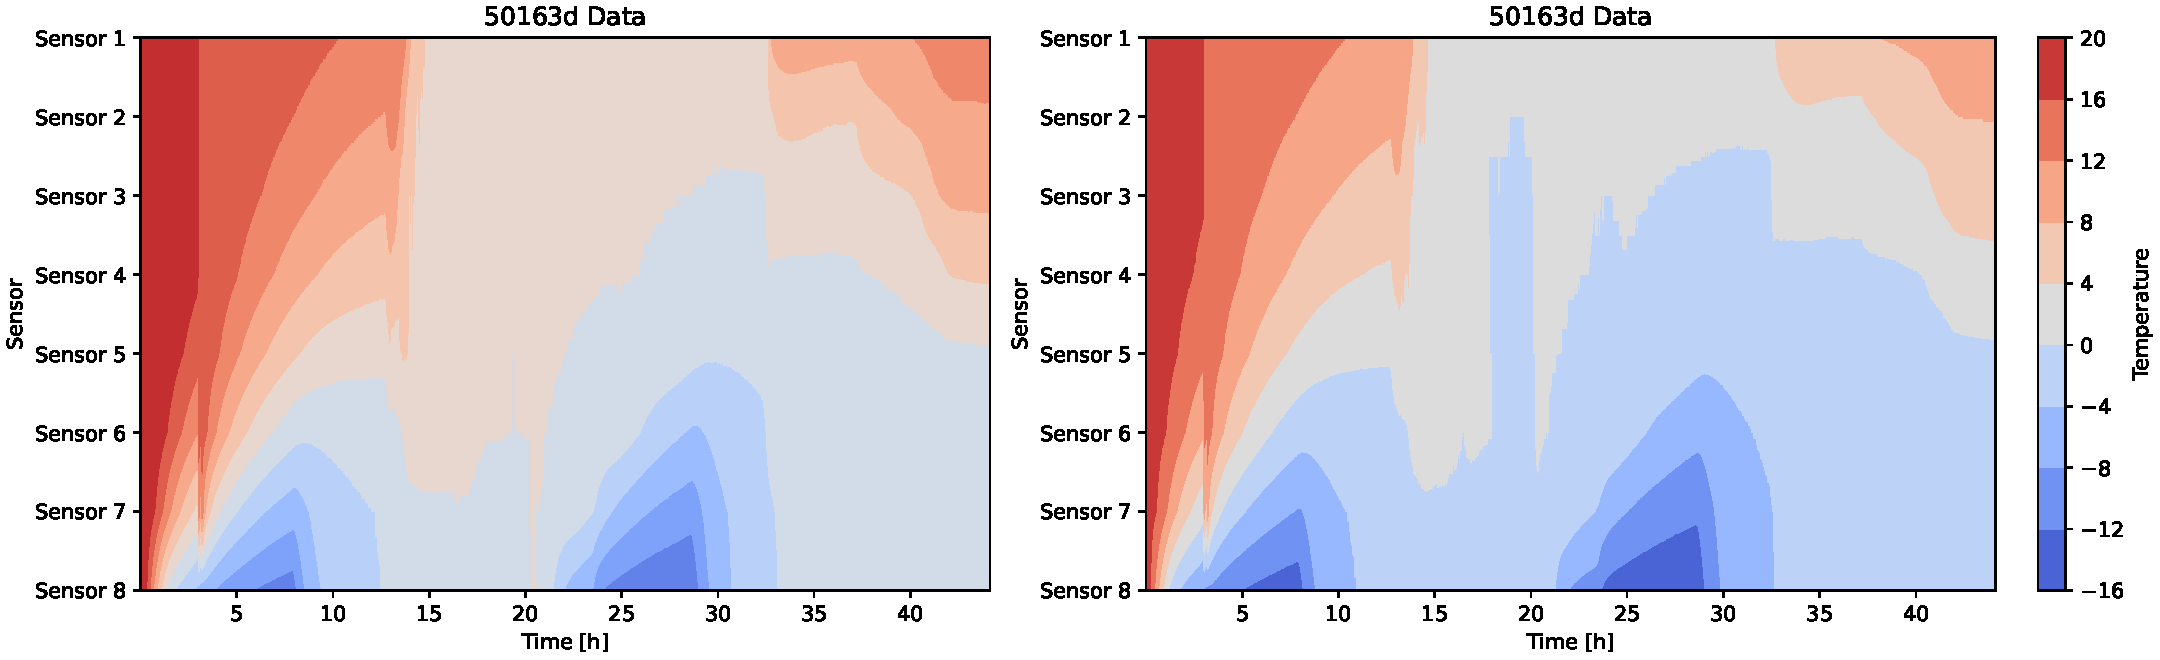
\includegraphics[width = 0.8\textwidth]{plots/plot1.pdf}
    \caption{Raw data from all sensors with timestamps plotted. It can be easily seen that sensor d39896f013c largely derivates from the other sensors in time. The other sensors mostly are very close with their timstamp with very small variations in time.}
    \label{fig:plot1}
\end{figure}
Figure \ref{fig:plot2} again shows the temperature data. A timestamp was added to the sensors that did not have a timestamp, according to the milliseconds recorded with the data. Also, using the df.diff() function of the panda package, the point at which the data drops off sharply (the point at which the sensors were placed in the water bath) was found and set to the same time point for all data. It can be seen that the data still has a systematic deviation in temperature and that each sensor has small differences in the time constant.\\

\begin{figure}
    \centering 
    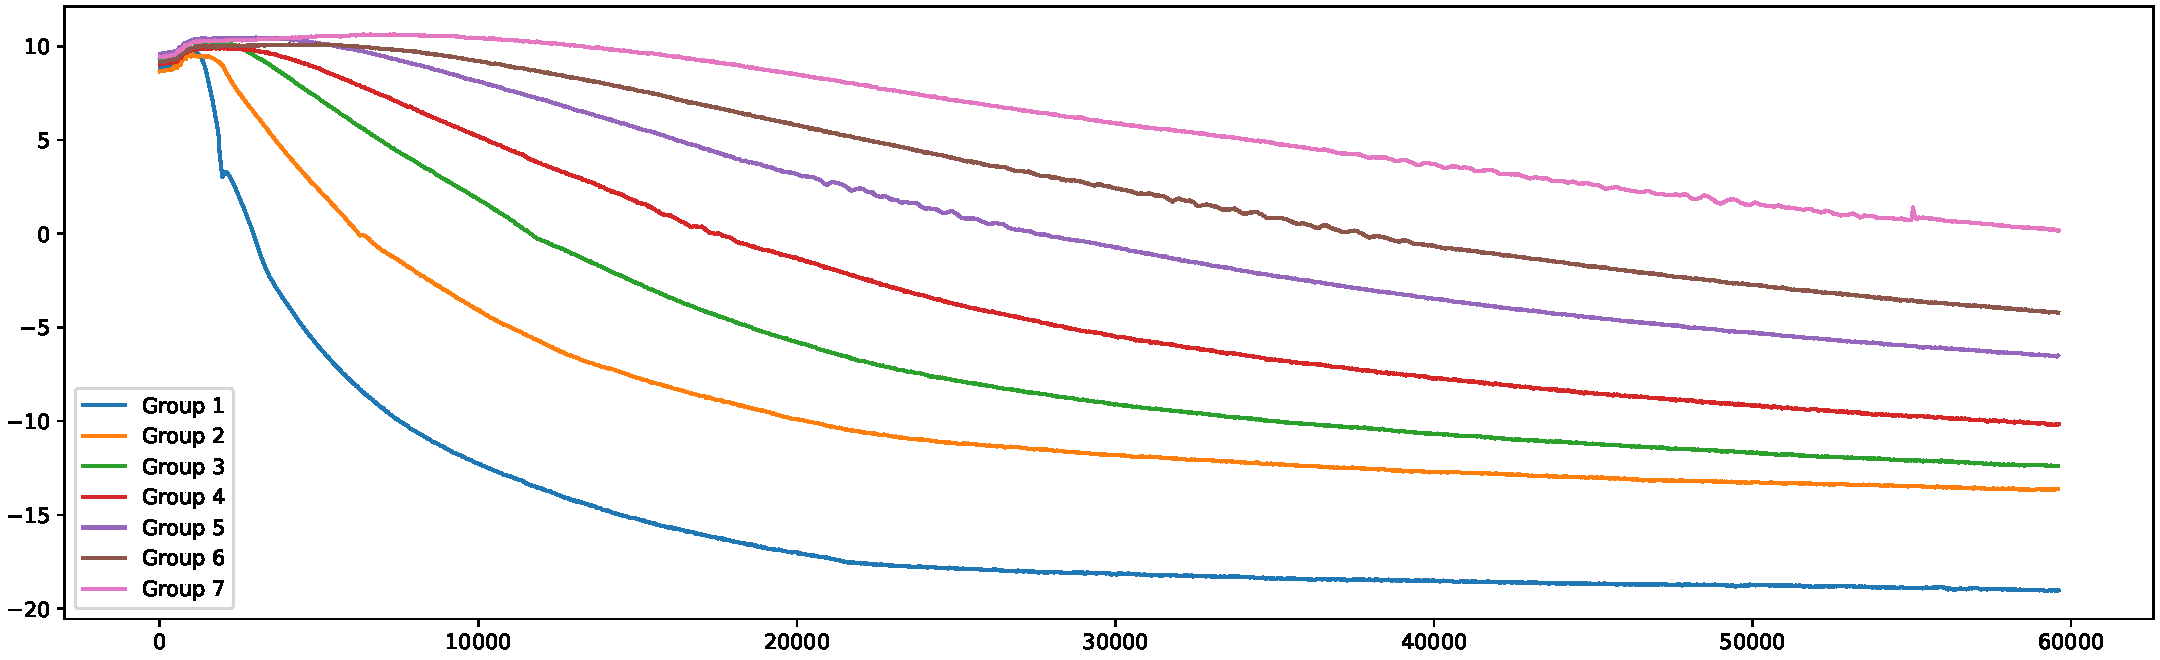
\includegraphics[width = 0.8\textwidth]{plots/plot2.pdf}
    \caption{The timestamp adjusted data of all Sensors. Apparently the data still varies in Temperature and the different sensors have different time constants.}
    \label{fig:plot2}
\end{figure}
In figure \ref{fig:plot4} the temperature data of the displacement sensors were calibrated. The difference between the measured temperature of the sensors and the measured temperature of the reference thermometer after immersing the two sensors in the water bath was determined.
The determined difference is then subtracted from the sensor values to calibrate them uniformly.
You can see that the values of the sensors differ only slightly from each other. \\

\begin{figure}
    \centering 
    \includegraphics[width = 0.8\textwidth]{plots/plot4.pdf}
    \caption{Rolling mean values of the temperature data and the temperature datapoints from the calibration measurement. The Values are adjusted with a calibration value at roughly 15:55 o'clock.}
    \label{fig:plot4}
\end{figure}
By showing the calibration data with \SI{0.5}{\celsius} added and remove with red lines in Figure \ref{fig:plot5} it can be seen that all values lay in the given accuracy of $\pm 0.5$ \si{\celsius}.\\

\begin{figure}
    \centering 
    \includegraphics[width = 0.8\textwidth]{plots/plot5.pdf}
    \caption{Just the rolling mean values while the thermometers are in the water bath. Withe red lines the deviation of 0.5 degree Celsius is shown.}
    \label{fig:plot5}
\end{figure}
To determine the time constant of the sensors, the value shortly before entering the water bath is compared with a value in the water bath and the difference is determined.
Then a cut-off value is determined at which the value has changed by at least \SI{63.2}{\percent}.
Finally, the time difference between the start and the cut-off value is determined and the mean value of all sensors is calculated.
According to the Gaussian error propagation, with an uncertainty of one second in the measured values, a value for the time constant of \SI{11(2.82)}{\second} results.
\begin{align}
    u_{time\_delta} &= \sqrt{1^2+(-1)^2)} = \sqrt{2}\\
    u_{avg\_time} &= \sqrt{(1/8*\sqrt{2})^2} = \sqrt{1/32} = 4\sqrt{0.5} ≈ 2.82843
\end{align}